%%%%%%%%%%%%%%%%%%%%%%%%%%%%%%%%%%%%%%%%%%%%%%%%%%%555
%From jm and nicolas frame 

  \newcommand{\mEDEA}{

	\begin{itemize}
		\item Each agent contains:
		\begin{itemize}
			\item an active genome, used to control the agent,
			\item a list of stored genomes, received during one generation.
		\end{itemize}
		
		\item At each time step, each agent:
		\begin{itemize}
			\item broadcasts a copy of its active genome,
			\item stores genomes received from neighboring agents.
		\end{itemize}
		
		\item At the end of the current generation, each agent:
		\begin{itemize}
			\item "forgets" its active genome,
			\item randomly selects one stored genome as new active genome and mutate it a little bit,
			\item empties the list of stored genomes.
		\end{itemize}
	\end{itemize}

}


%------------------------------------------------------------
\begin{frame}{The "mEDEA" Algorithm}
\begin{figure}
 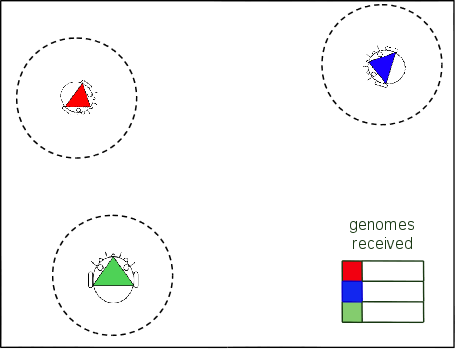
\includegraphics[height=3cm]{images/medea0}
\end{figure}

  \mEDEA

\end{frame}

%------------------------------------------------------------
\begin{frame}{The "mEDEA" Algorithm}\addtocounter{framenumber}{-1}
\begin{figure}
 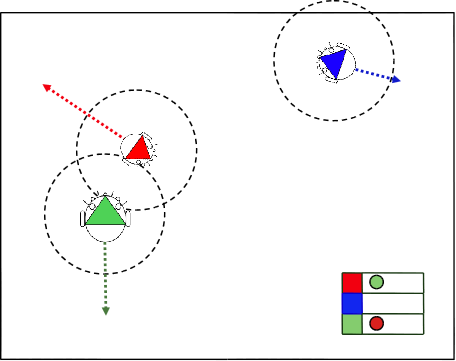
\includegraphics[height=3cm]{images/medea1}
\end{figure}
   \mEDEA
\end{frame}
%------------------------------------------------------------
\begin{frame}{The "mEDEA" Algorithm}\addtocounter{framenumber}{-1}
\begin{figure}
 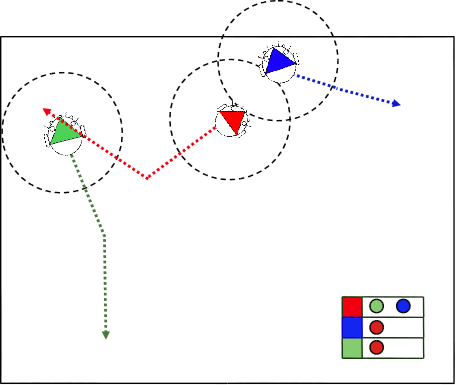
\includegraphics[height=3cm]{images/medea2}
\end{figure}
   \mEDEA
\end{frame}

%------------------------------------------------------------

\begin{frame}{The "mEDEA" Algorithm}\addtocounter{framenumber}{-1}
\begin{figure}
 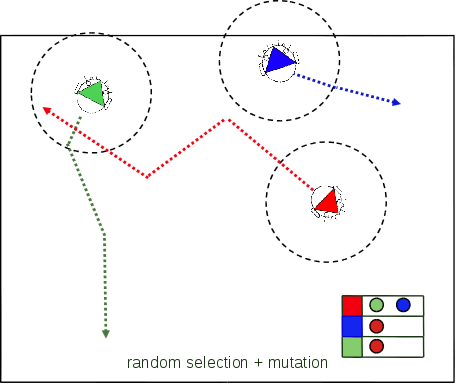
\includegraphics[height=3cm]{images/medea3}
\end{figure}
   \mEDEA
\end{frame}


%%%%%%%%%%%%%%%%%%%%%%%%%%%%%%%%%%


